\chapter{Overview}
\label{cha:overview}

This chapter gives informal introduction to the RFSM language and of how to use it to describe 
FSM-based systems.

\section{Introductory example}
\label{sec:first-example}

Listing~\ref{lst:rfsm-gensig} is an example of a simple RFSM program\footnote{This program is
  provided in the distribution, under directory \texttt{examples/single/gensig/v2}.}. This program is
used to describe and simulate the model of a calibrated pulse generator. Given an input clock
\verb|H|, with period $T_H$, it generates a pulse of duration $n \times T_H$ whenever input
\texttt{E} is set when event $H$ occurs.

\begin{lstlisting}[language=Rfsm,frame=single,numbers=left,caption=A simple RFSM
  program,label={lst:rfsm-gensig},float]
@\label{gensig-1a}@fsm model gensig <n: int> (
  in h: event,
  in e: bool,
  out s: bool)
{
  states: E0, E1;
@\label{gensig-3}@  vars: k: int<0:n>;
  trans:
  | E0 -> E1 on h when e=1 with k:=1,s:=1
@\label{gensig-4}@  | E1 -> E1 on h when k<n with k:=k+1
@\label{gensig-5}@  | E1 -> E0 on h when k=n with s:=0;
  itrans:
  | -> E0 with s:=0;
@\label{gensig-1b}@}

@\label{gensig-2a}@input H : event = periodic (10,0,80)
input E : bool = value_changes (0:0, 25:1, 35:0)
@\label{gensig-2b}@output S : bool 

@\label{gensig-6}@fsm g = gensig<4>(H,E,S)
\end{lstlisting}

The program can be divided in four parts.

\medskip The first part (lines \ref{gensig-1a}--\ref{gensig-1b}) gives a \textbf{generic model} of
the generator behavior. The model, named \verb|gensig|, has one parameter, \verb|n|, two inputs,
\verb|h| and \verb|e|, of type \verb|event| and \verb|bool| respectively, and one output \verb|s| of
type \verb|bool|. Its behavior is specified as a reactive FSM with two states, \verb|E0| and
\verb|E1|, and one internal variable \verb|k|. The transitions of this FSM are given after the
\verb|trans:| keyword in the form :
\begin{center}
  \framebox{\lstinline[language=Rfsm]{| source_state -> destination_state on ev when guard with
    actions}}
\end{center}
where
\begin{itemize}
\item \emph{ev} is the event trigerring the transition,
\item \emph{guard} is a set of (boolean) conditions,
\item \emph{actions} is a set of actions performed when the transition is enabled.
\end{itemize}
The semantics is that the transition is enabled
whenever the FSM is in the source state, the event \emph{ev} occurs and all the conditions in the
guard are true. The associated actions
are then performed and the FSM moves to the destination state. For example, the first transition is
enabled whenever an event occurs on input \verb|h| and, at this instant, the value of input \verb|e|
is 1. The FSM then goes from state \verb|E0| to state \verb|E1| and sets its internal variable 
\verb|k| and its output \verb|s| to 1. The \emph{initial transition} of the FSM is given 
after the \verb|itrans:| keyword in the form :
\begin{center}
  \framebox{\lstinline[language=Rfsm]{| -> initial_state with actions}}
\end{center}
Here the FSM is initially in state \verb|E0| with output \verb|s| set to 0.

A graphical representation of the \verb|gensig| model is given in
Fig.~\ref{fig:rfsm-gensig-model} (this representation was actually automatically generated from the
program in Listing~\ref{lst:rfsm-gensig}, as explained in Chap.~\ref{cha:rfsmc}). 

\begin{figure}[!h]
   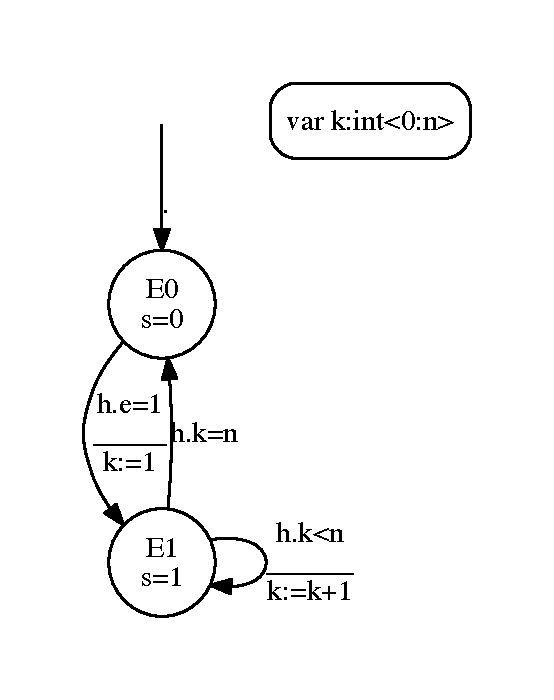
\includegraphics[height=8cm]{figs/gensig-model}
   \centering
  \caption{A graphical representation of FSM model defined in Listing~\ref{lst:rfsm-gensig}}
  \label{fig:rfsm-gensig-model}
\end{figure}

Note that, at this level, the value of the parameter \verb|n|, used in the type of the internal
variable \verb|k| (line~\ref{gensig-3}) and in the transition conditions (lines \ref{gensig-4} and
\ref{gensig-5}) is left unspecified, making the \verb|gensig| model a \emph{generic} one.

\medskip The second part of the program (lines \ref{gensig-2a}--\ref{gensig-2b}) lists \textbf{global inputs and
  outputs}\footnote{In case of multi-FSM programs, this part will also contains the declaration of
  \emph{shared} events and variables. See Sec.~\ref{sec:globals}.}.  For global outputs the
declaration simply gives a name and a type.  For global inputs, the declaration also specifies the
\textbf{stimuli} which are attached to the corresponding input for simulating the system. The
program of Listing~\ref{lst:rfsm-gensig} uses two kinds of stimuli\footnote{See
  Sec.~\ref{sec:globals} for a complete description of stimuli.}. The stimuli attached to input
\verb|H| are declared as \emph{periodic}, with a period of 10 time units, a start time of 0 and a
end time of 80. This means than an event will be produced on this input at time 0, 10, 20, 30, 40,
50, 60, 70 and 80. The stimuli attached to input \verb|E| say that this input will respectively take
value 0, 1 and 0 at time 0, 25 and 35 (thus producing a ``pulse'' of duration 10 time units starting
at time 25).

\medskip
The third and last part of the program (line~\ref{gensig-6}) consists in building the global model of the system by
\emph{instanciating} the FSM model(s).
Instanciating a model creates a ``copy'' of this model for which
\begin{itemize}
\item the generic parameters (\verb|n| here) are now bound to actual values (4 here),
\item the inputs and outputs are connected to the global inputs or outputs. 
\end{itemize}

\medskip
A graphical representation of the system described in Listing~\ref{lst:rfsm-gensig} is given in
Fig.~\ref{fig:rfsm-gensig-top}\footnote{Again, this representation was actually automatically generated from the
program in Listing~\ref{lst:rfsm-gensig}, as explained in Chap.~\ref{cha:rfsmc}}. 

\begin{figure}[!h]
   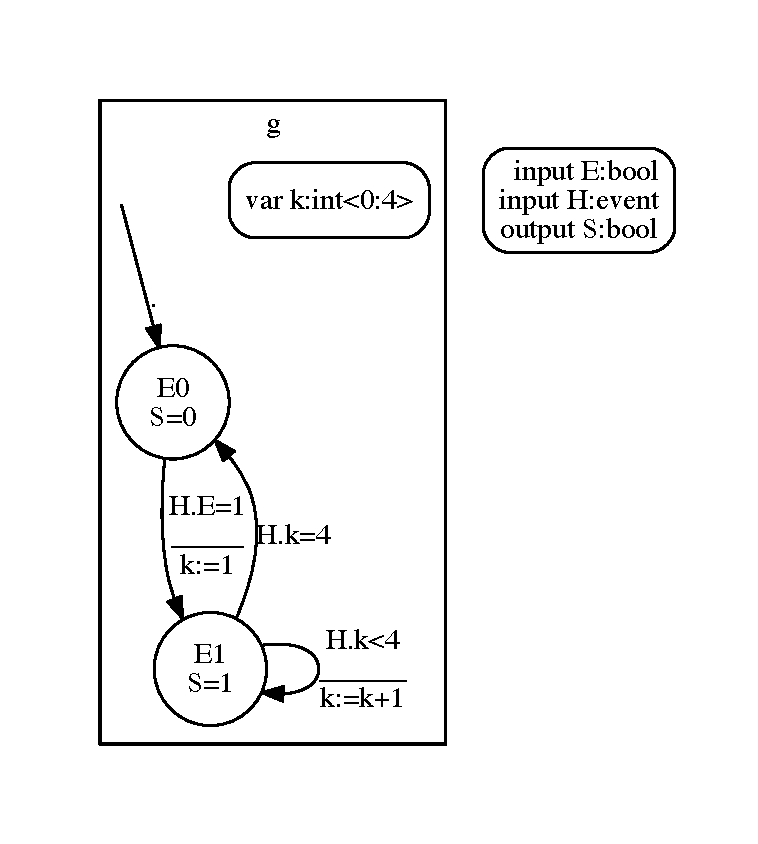
\includegraphics[height=8cm]{figs/gensig-top}
   \centering
  \caption{A graphical representation of system described in Listing~\ref{lst:rfsm-gensig}}
  \label{fig:rfsm-gensig-top}
\end{figure}

\subsection*{Simulating}
\label{sec:simulating-1}

Simulating the program means computing the reaction of the system to the input stimuli. Simulation
can be performed the RFSM command-line compiler or the IDE (see Chap.~\ref{cha:rfsmc} and \ref{cha:gui} resp.).
It produces a set of
\emph{traces} in VCD (Value Change Dump) format which can visualized using \emph{waveform viewers}
such as \texttt{gtkwave}. The simulation results for the program in Listing~\ref{lst:rfsm-gensig}
are illustrated in Fig.~\ref{fig:rfsm-gensig-chrono}.

\begin{figure}[!h]
   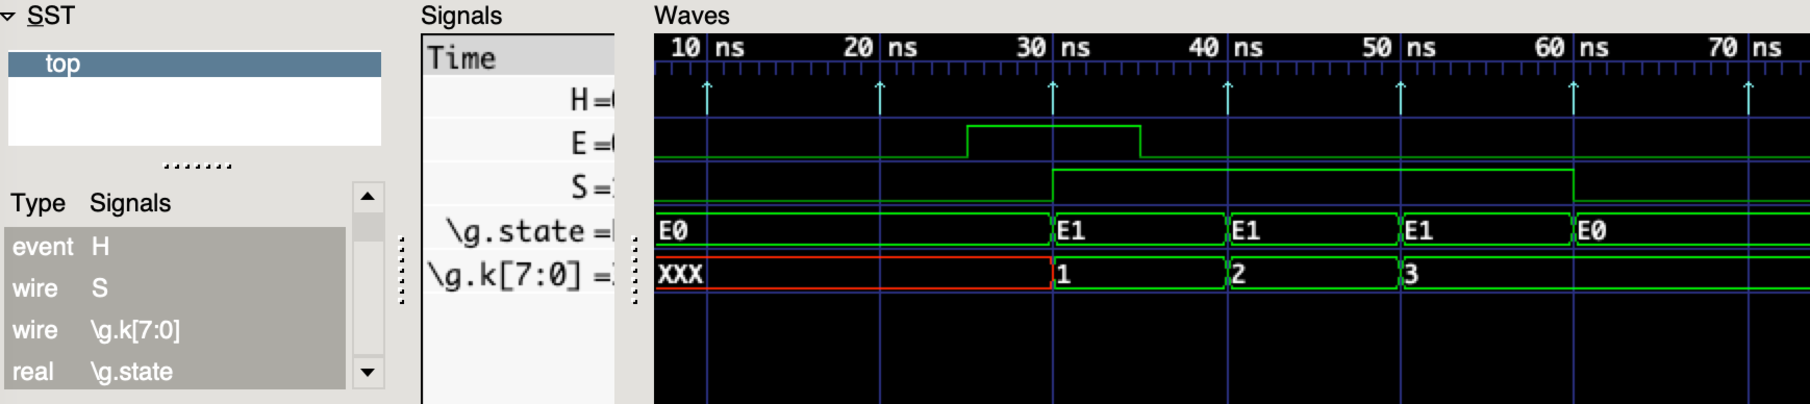
\includegraphics[width=\textwidth]{figs/gensig-chrono}
   \centering
  \caption{Simulation results for the program in Listing~\ref{lst:rfsm-gensig}, viewed using
    \texttt{gtkwave}}
  \label{fig:rfsm-gensig-chrono}
\end{figure}

\subsection*{Code generation}
\label{sec:code-generation-1}

RFSM can also generate code implementing the described systems simulation and/or
integration to existing applications.

\medskip
Currently, three backends are provided :
\begin{itemize}
\item a backend generating a C-based implementation of each FSM instance,
\item a backend generating a \emph{testbench} implementation in SystemC (FSM instances + stimuli
  generators),
\item a backend generating a \emph{testbench} implementation in VHDL (FSM instances + stimuli
  generators).
\end{itemize}

\medskip
The target language for the C backend is a C-like language augmented with
\begin{itemize}
\item a \verb|task| keyword for naming generated behaviors,
\item \verb|in|, \verb|out| and \verb|iinout| keywords for identifying inputs and outputs,
\item a builtin \verb|event| type,
\item primitives for handling events : \verb|wait_ev()|, \verb|wait_evs()| and
  \verb|notify_ev()|. 
\end{itemize}
The idea is that the generated code can be turned into an application for a multi-tasking operating
system by providing actual implementations of the corresponding constructs and primitives.

\medskip
For the SystemC and VHDL backends, the generated code can actually be compiled and executed for
simulation purpose and. The FSM implementations generated by the VHDL backend can also be
synthetized to be implemented hardware using hardware-specific tools\footnote{We use the
  \textsc{quartus} toolchain from Intel/Altera.}. 

\medskip
Appendices C1, C2 and C3 respectively give the C and SystemC code generated from the example in
Listing~\ref{lst:rfsm-gensig}. 

\subsection*{Variant formulation}
\label{sec:variant-formulation}

In the automata described in Fig.~\ref{fig:rfsm-gensig-model} and Listing~\ref{lst:rfsm-gensig}, the
\texttt{s} output is defined by modifiying its value when some transitions are taken (namely,
\texttt{s} is set to 0 on the initial transition and on the transition from \texttt{E1} to
\texttt{E0} and set to 1 on the transition from \texttt{E0} to \texttt{E1}). This is typical of a
so-called \emph{Mealy}-style description. Sometimes, a description in which the value of the outputs
are attached to \texttt{states} rather than to transitions is more natural. This style of
description, often called \emph{Moore}-style, is illustrated in Fig.~\ref{fig:rfsm-gensig-moore} and
Listing~\ref{lst:rfsm-gensig-moore} for the calibrated pulse generator. Associating the value of the
\texttt{s} output to the states is done line~\ref{gensigm-1}, using the \texttt{where}
clause. Correlatively, the update of this output have been removed from the actions attached to the
transitions described lines~\ref{gensigm-2a}, \ref{gensigm-2b} and \ref{gensigm-3}.

\begin{figure}[!h]
   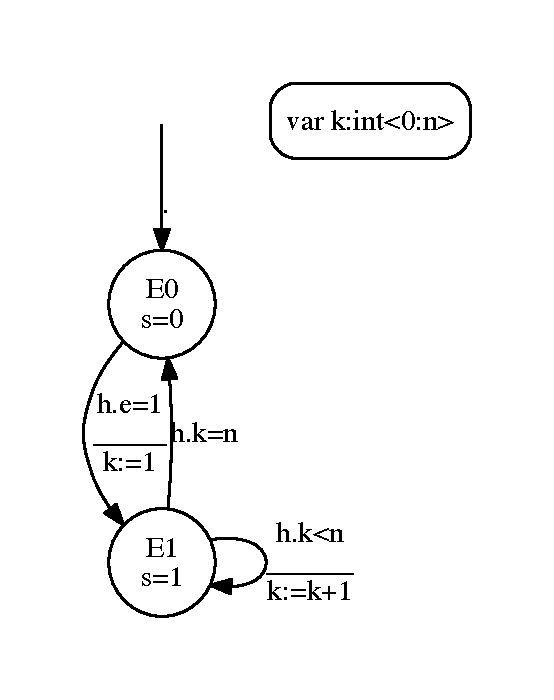
\includegraphics[height=7cm]{figs/gensig-model}
   \centering
  \caption{A Moore-style reformulation of the model defined in Fig.~\ref{fig:rfsm-gensig-model}}
  \label{fig:rfsm-gensig-moore}
\end{figure}


\begin{lstlisting}[language=Rfsm,frame=single,numbers=left,caption=Transcription in RFSM of the
  model given in Fig.~\ref{fig:rfsm-gensig-moore},label={lst:rfsm-gensig-moore},float]
fsm model gensig <n: int> (
  in h: event,
  in e: bool,
  out s: bool)
{
@\label{gensigm-1}@  states: E0 where s=0, E1 where s=1;
  vars: k: int<0:n>;
  trans:
@\label{gensigm-2a}@  | E0 -> E1 on h when e=1 with k:=1
  | E1 -> E1 on h when k<n with k:=k+1
@\label{gensigm-2b}@  | E1 -> E0 on h when k=n
  itrans:
@\label{gensigm-3}@  | -> E0
}
\end{lstlisting}

\clearpage
\section{The RFSM language}
\label{sec:rfsm-language}

This section is more thorough presentation of the RFSM language introduced in the previous
section. This presentation is deliberately informal. The complete language syntax can
be found in Appendix~A.

\subsection{Types}
\label{sec:types}

There are two categories of types~: builtin types and user defined types.

\medskip
\textbf{Builtin types} are : \texttt{bool}, \texttt{int}, \texttt{float}, \texttt{char}, \texttt{event} and
\texttt{array}s.

\step Objects of type \texttt{bool} can have only two values : \texttt{0} (false) and \texttt{1} (true).

\step Values of type \texttt{char} are
denoted using single quotes. For example, for a variable \verb|c| having type \verb|char| :
\begin{center}
  \example{\lstinline[language=Rfsm]|c := 'A'|}
\end{center}
They can be converted from/to they internal representation as integers using the "\verb|::|" \emph{cast}
operator. For example, if \verb|c| has type \verb|char| and \verb|n| type \verb|int|, then 
\begin{center}
  \example{\lstinline[language=Rfsm]|n := 'A'::int; c:=(n+1)::char|}
\end{center}
assigns value 65 to \verb|n| (ASCII code) and, then, value \verb|'B'| to \verb|c|.


\step The type \texttt{int} can be refined using a \emph{size} or a \emph{range annotation}. The
type \verb|int<sz>|, where \verb|sz| is an integer, is the type of integers which can be encoded using
\verb|n| bits. The type \verb|int<min:max>|, where both \verb|min| and \verb|max| are integers, is
the type of integers whose value ranges from \verb|min| to \verb|max|. The size and range limits,
can be constants or expressions whose value can be computed as compile time
(expressions involving parameter values, as exemplified line 9 in Listing~\ref{lst:rfsm-gensig}).

\step Supported operations on values of type \texttt{int} are described in Table~\ref{tab:int-ops}.
If \verb|n| is an integer and \verb|hi| (resp. \verb|lo|) an integer expression then \verb|n[hi:lo]|
designates the value represented by the bits \verb|hi|...\verb|lo| in the binary representation of
\verb|n|. Bit ranges can be both read (ex: \verb|x=y[6:2]|) or written (ex: \verb|x[8:4]:=0|). The
syntax \verb|n[i||, where \verb|n| is an integer is equivalent to \verb|n[i:i]|. The \emph{cast}
operator (\verb|::|) can be used to combine integers with different sizes (for example, if \verb|n|
has type \verb|int<16>| and \verb|m| has type \verb|int<8>|, writing \verb|n:=n+m| is not allowed
and mus be written, instead, \verb|n:=n+m::int<16>|. Note that the
logical ``or'' operator is denoted ``\verb+||+'' because the single ``\verb+|+'' is already used in
the syntax.

\begin{table}
\begin{center}
\begin{tabular}{|l|l|} \hline
\verb|+|, \verb|-|, \verb|*|, \verb|/|, \verb|%| (modulo) & arithmetic operations \\ \hline 
\verb|>>|, \verb|<<| & (logical) shift right and left \\ \hline 
\verb|&|, \verb+||+, \verb|^| & bitwise and, or and xor \\ \hline 
\verb|[.:.]| & bit range extraction (ex: \verb|n:=m[5:3]|) \\ \hline 
\verb|[.]| & single bit extraction (ex: \verb|b:=m[4]|) \\ \hline 
\verb|::| & resize (ex: \verb|n::8|) \\ \hline 
\end{tabular}
\caption{\label{tab:int-ops}Builtin operations on integers}
\end{center}
\end{table}

\step The operations on values of type \texttt{float} are : "\verb|+.|", "\verb|-.|", "\verb|*.|" and
"\verb|/.|" (the dot suffix is required to distinguish them from the corresponding operations on
\texttt{int}s).


\step Arrays are 1D, fixed-size collections of \verb|int|s, \verb|bool|s or \verb|float|s. Indices
range from 0 to \verb|n-1| where \verb|n| is the size of the array. For example,
 \verb|int array[4]| is the type describing arrays of four integers. If \verb|t| is an object
  with an array type, its cell with index $i$ is denoted \verb|t[i]|.


\medskip
\textbf{User defined types} are either \emph{type abbreviations}, \emph{enumerations} or
\emph{records}.

\step Type abbreviations are introduced with the following declaration
\begin{center}
  \framebox{\lstinline[language=Rfsm]{type typename = type_expression}}
\end{center}
Each occurrence of the defined type in the program is actually substituted by the corresponding type
expression.
% Type expressions in type abbreviations are currently limited to builtin types.

\medskip
\step Enumerated types  are introduced with the following declaration
\begin{center}
  \framebox{\lstinline[language=Rfsm]|type typename = enum \{ C1, ..., Cn \}|}
\end{center}
where \verb|C1|, \ldots, \verb|Cn| are the enumerated values, each being denoted by an identifier
starting with an uppercase letter. For example : 
\begin{center}
  \example{\lstinline[language=Rfsm]|type color = \{ Red, Green, Orange \}|}
\end{center}

\medskip
\step Record types are introduced with the following declaration
\begin{center}
  \framebox{\lstinline[language=Rfsm]|type typename = record \{ fid1: ty1, ..., fidn: tyn \}|}
\end{center}
where \verb|fid1|, \ldots, \verb|fidn| and \verb|ty1|, \ldots, \verb|tyn| are respectively the name
and type of each record field For example : 
\begin{center}
  \example{\lstinline[language=Rfsm]|type coord = record \{ x: int, y: int\}|}
\end{center}

Individual fields of a value with a record type can be accessed using the classical ``dot''
notation. For example, with a variable \verb|c| having type \verb|record| as defined above :
\begin{center}
  \example{\lstinline[language=Rfsm]|c.x := c.x+1|}
\end{center}


\subsection{FSM models}
\label{sec:fsm-models}

An FSM model, introduced by the \verb|fsm model| keywords, describes the interface and behavior of a
\emph{reactive finite state machine}. A reactive finite state machine is a finite state machine
whose transitions can only be caused by the occurrence of \emph{events}.

\begin{center}
\framebox{\lstinline[language=Rfsm]|fsm model <interface> { <body> }|}
\end{center}

\medskip
The \textbf{interface} of the model gives its name, a list of parameters (which can be empty) and a
list of inputs and outputs. All parameters and IOs are typed. Inputs and outputs are explicitely
tagged. An IO tagged \verb|inout| acts both as input and output (it can be read and written by the
model). Inputs and outputs are listed between \verb|(...)|. Parameters, if present are given between
\verb|<...>|. Examples :

\begin{center}
\example{\lstinline[language=Rfsm]|fsm model cntmod8 (in h: event, out s: int<0..7>) \{ ... \}|}
\end{center}

\begin{center}
\example{\lstinline[language=Rfsm]|fsm model gensig<n:int> (in h: event, in  e: bit, out s: bit) \{ ... \}|}
\end{center}

\begin{center}
\example{\lstinline[language=Rfsm]|fsm model update (in top: event, inout  lock: bool) \{ ... \}|}
\end{center}

\medskip
The model \textbf{body}, written between \verb|{...}|, generally comprises four sections :
\begin{itemize}
\item a section giving the list of \emph{states},
\item a section introducing local (internal) \emph{variables},
\item a section giving the list of \emph{transition},
\item a section specifying the \emph{initial transition}.
\end{itemize}

Each section starts with the corresponding keyword (\verb|states:|, \verb|vars:|, \verb|trans:| and
\verb|itrans:| resp.) and ends with a semi-colon.

\begin{center}
\framebox{\lstinline[language=Rfsm]| fsm model ... ( ... ) \{ states: ...; vars: ...; trans: ...; itrans: ...; \}|}
\end{center}

\subsubsection*{States}
\label{sec:states}

The \verb|states:| section gives the set of internal states, as a comma-separated list of
identifiers (each starting with a uppercase letter). Example :

\begin{center}
\example{\lstinline[language=Rfsm]|states: Idle, Wait1, Wait2, Done;|}
\end{center}

Values for outputs can be attached to states using the \verb|where| keyword.

\begin{center}
\example{\lstinline[language=Rfsm]|states: Idle, Wait1 where s1=0, Wait2 where s1=1,s2=0, Done;|}
\end{center}

\subsubsection*{Variables}
\label{sec:variables}

The \verb|vars:| section gives the set of internal variables, each with its type. Example :

\begin{center}
\example{\lstinline[language=Rfsm]|vars: cnt: int, stop: bool;|}
\end{center}

The type of a variable may depend on parameters listed in the model interface. Example

\begin{center}
\example{\lstinline[language=Rfsm]|fsm gensig<n: int> (...) \{ ... vars: k: int<0..n>; ... \}|}
\end{center}

The \verb|vars:| section may be omitted.

\subsubsection*{Transitions}
\label{sec:transitions}

The \verb|trans:| section gives the set of transitions between states. Each transition is denoted

\begin{center}
\framebox{\lstinline[language=Rfsm]{| src_state -> dst_state on ev when guards with actions}}
\end{center}

where
\begin{itemize}
\item \emph{src\_state} and \emph{dst\_state} respectively designates the source state and destination state,
\item \emph{ev} is event trigerring the transition,
\item \emph{guards} is a set a enabling conditions,
\item \emph{actions} is a set of actions performed when then transition is enabled.
\end{itemize}

\medskip The semantics is that the transition is enabled whenever the FSM is in the source state,
the triggering event occurs and all conditions evaluate to true. The associated actions are then
performed and the FSM moves to the destination state.

\medskip
The triggering event must be listed in the inputs.

\medskip
Each condition listed in \emph{guards} must evaluate to a boolean value. The guard is true if
\emph{all} conditions evaluate to true (conjonctive semantics).
The guards may involve inputs and/or internal variables.

\medskip
The guard can be empty. In this case, the transition is denoted
\begin{center}
\framebox{\lstinline[language=Rfsm]{| src_state -> dst_state on ev with actions}}
\end{center}

\medskip The \textbf{actions} associated to a transition consists in modifications of the outputs
and/or internal variables or emissions of events. Modifications of outputs and internal variables
are denoted

\begin{center}
\framebox{\lstinline[language=Rfsm]{id := expr}}
\end{center}

where \emph{id} is the name of the output (resp. variable) and \emph{expr} an expression involving
inputs, outputs and variables and operations allowed on the corresponding types. The set of allowed
operations is given in Table~\ref{tab:type-ops}.

\begin{table}
\begin{minipage}[c]{1.0\linewidth}
\small
\begin{center}
\begin{tabular}{|l|l|} \hline
{\tt int}       & {\tt + - * / mod = != > < >= <=} \\  \hline
{\tt bool}      & {\tt = !=} \\ \hline 
{\tt enumeration}     & {\tt = !=} \\  \hline
\end{tabular}
\caption{Operations on types}
\label{tab:type-ops}
\end{center}
\end{minipage}
\end{table}

\medskip
The action of emitting of an event  is simply denoted by the name of this event.

\medskip
Examples :

\begin{center}
\example{\lstinline[language=Rfsm]'S0 -> S1 on top '}
\end{center}

In the above example, the enclosing FSM switches from state \verb|S0| to state \verb|S1| when the
event \verb|top| occurs. 

\begin{center}
\example{\lstinline[language=Rfsm]'Idle -> Wait on Clic with ctr:=0, received'}
\end{center}

In the above example, the enclosing FSM switches from state \verb|Idle| to state \verb|Wait|, resetting the internal variable
  \verb|ctr| to 0 and emitting event \verb|received| whenever an event occurs on its \verb|Clic| input.

\begin{center}
\example{\lstinline[language=Rfsm]'Wait -> Wait on Top when ctr<8 with ctr:=ctr+1'}
\end{center}

In the above example, the enclosing FSM stays in state \verb|Wait| but increments the internal
variable \verb|ctr| whenever an event \verb|Top| occurs and that, \emph{at this instant}, the
value of variable \verb|ctr| is smaller than 8. 

\medskip
Expressions may also involve the C-like ternary conditional operator \verb|?:|.
For example, in the example below, the enclosing FSM stays in state \verb|S0| but updates the variable \verb|k|
at each occurrence of event \verb|H| so that is incremented if its current value is less than 8 or
reset to 0 otherwise.

\begin{center}
\example{\lstinline[language=Rfsm]'S0 -> S0 on H with k:=k<8?k+1:0'}
\end{center}

\medskip
The set of actions may be empty. In this case, the transition is denoted :

\begin{center}
\framebox{\lstinline[language=Rfsm]{src_state -> dst_state on ev when guard}}
\end{center}

\subsubsection*{Initial transition}
\label{sec:initial-transition}

The \verb|itrans:| section specifies the initial transition of the FSM. This transition is denoted~:

\begin{center}
\framebox{\lstinline[language=Rfsm]{| -> init_state with actions}}
\end{center}

where \emph{init\_state} is the initial state and \emph{actions} a list of actions to be performed
when initializing the FSM. The latter can be empty. in this case the initial transition is simply
denoted~:

\begin{center}
\framebox{\lstinline[language=Rfsm]{| -> init_state}}
\end{center}

\medskip
\textbf{Note}. Output values can be set by either attaching them to states or by updating them on
transitions. For a given output \texttt{o}, attaching a value \texttt{v} to a state \texttt{S}, by writing

\begin{center}
\framebox{\lstinline[language=Rfsm]{states: S where o=v, ...}}
\end{center}

is equivalent to adding the action

\begin{center}
\framebox{\lstinline[language=Rfsm]{o:=v}}
\end{center}

to each transition ending at state \texttt{S}.

The semantics of a model in which the value of an output deduced from the former formulation is
different from that deduced from the latter is undefined. This condition is statically
undecidable in general. This said, the RFSM compiler emits a warning when both formulations are
present in a given model for a given output.

\subsection{Globals}
\label{sec:globals}

Globals are used to connect model instances to the external world or to other instances.

\subsubsection*{Inputs and outputs}
\label{sec:inputs-outputs}

Interface to the external world are represented by \verb|input| and \verb|output| objects.

\step For outputs the declaration simply gives a name and a type~:

\begin{center}
\framebox{\lstinline[language=Rfsm]'output name : typ'}
\end{center}

\step For inputs, the declaration also specifies the \textbf{stimuli} which are attached to the
corresponding input for simulating the system.
\begin{center}
\framebox{\lstinline[language=Rfsm]'input name : typ = stimuli'}
\end{center}

There are three types of stimuli~:
periodic and
sporadic stimuli for inputs of type \verb|event| and value changes for scalar inputs.

\medskip
Periodic stimuli are specified with a period, a starting time and an ending time.

\begin{center}
\framebox{\lstinline[language=Rfsm]'periodic(period,t0,t1)'}
\end{center}

Sporadic stimuli
are simply a list of dates at which the corresponding input event occurs.

\begin{center}
\framebox{\lstinline[language=Rfsm]'sporadic(t1,...,tn)'}
\end{center}

Value changes are given as
list of pairs \verb|t:v|, where \verb|t| is a date and \verb|v| the value assigned to the
corresponding input at this date. 

\begin{center}
\framebox{\lstinline[language=Rfsm]'value_changes(t1:v1,...,tn:vn)'}
\end{center}

\medskip
Examples:

\begin{center}
\example{\lstinline[language=Rfsm]'input Clk: event = periodic(10,10,120)'}
\end{center}

The previous declaration declares \verb|Clk| as a global input producing periodic events with period 10, starting
  at t=10 and ending at t=100\footnote{Note that, at this level, there's no need for an absolute
    unit for time.}.

\begin{center}
\example{\lstinline[language=Rfsm]'input Clic: event = sporadic(25,75,95)'}
\end{center}

The previous declaration declares \verb|Clic| as a global input producing events at t=25, t=75 and
  t=95.

\begin{center}
\example{\lstinline[language=Rfsm]'input E : bool = value_changes (0:false, 25:true, 35:false)'}
\end{center}

The previous declaration declares \verb|E| as a global boolean input taking value \texttt{false} at
t=0, \texttt{true} at t=25 and \texttt{false} again at t=35.

\subsubsection*{Shared objects}
\label{sec:shared}

Shared objects are used to represent interconnexions between FSM instances. This situation only
occurs when the system model involves several FSM instances and when the input of a given instance
is provided by the output of another one (see Section~\ref{sec:fsm-instances}).

\step For shared objects the declaration simply gives a name and a type~:

\begin{center}
\framebox{\lstinline[language=Rfsm]'shared name : typ'}
\end{center}

\subsection{Instances and system}
\label{sec:fsm-instances}

The description of the system is carried out by instanciating
-- and, possibly, inter-connecting -- previously defined FSM models.

\medskip
Instanciating a model creates a ``copy'' of the corresponding FSM for which
\begin{itemize}
\item the parameters of the model are bound to their actual value,
\item the declared inputs and outputs are connected to global inputs, outputs or shared
  objects.
\end{itemize}

\medskip
The syntax for declaring a model instance is as follows~:

\begin{center}
\framebox{\lstinline[language=Rfsm]'fsm inst_name = model_name<param_values>(actual_ios)'} 
\end{center}

where
\begin{itemize}
\item \emph{inst\_name} is the name of the created instance,
\item \emph{model\_name} is the name of the instanciated model,
\item \emph{param\_values} is a comma-separated list of values to be assigned to the formal
  (generic) parameters,
\item \emph{actual\_ios} is a comma-separated list of global inputs, outputs or shared objects to be
  connected to the instanciated model.
\end{itemize}

Binding of parameter values and IOs is done by position. Of course the number and respective types
of the formal and actual parameters (resp. IOs) must match.

\medskip
For example, the last line of the program given in Listing~\ref{lst:rfsm-gensig}

\begin{center}
\example{\lstinline[language=Rfsm]'fsm g = gensig<4>(H,E,S)'}
\end{center}

creates an instance of model \verb|gensig| for which \verb|n=4| and whose inputs (resp. output) are
connected to the global inputs (resp. output) \texttt{H} and \texttt{E} (resp. \texttt{S}).

\subsubsection*{Multi-FSM models}
\label{sec:multi-fsm-models}

It is of course possible to build a system model as a \emph{composition} of FSM instances.  An
example is given in Listing~\ref{lst:rfsm-cntmod8}. The system is a simple modulo 8 counter, here
described as a combination of three event-synchronized modulo 2 counters\footnote{This program is
  provided in the distribution, under directory \texttt{examples/multi/ctrmod8}.}.

\medskip
Here a single FSM model (\texttt{cntmod2}) is instanciated thrice, as \texttt{C0}, \texttt{C1} and
\texttt{C2}. These instances are synchronized using two \textbf{shared events}, \texttt{R0} and \texttt{R1}. 

\medskip
The graphical representation of the program is given in Fig.~\ref{fig:rfsm-cntmod8-top}. Simulation
results are illustrated in Fig~\ref{fig:rfsm-cntmod8-vcd}. 

\begin{lstlisting}[language=Rfsm,frame=single,numbers=left,caption=A multi-model RFSM
  program,label={lst:rfsm-cntmod8},float]
fsm model cntmod2(
  in h: event,
  out s: int<0:1>,
  out r: event)
{
  states: E0, E1;
  trans:
  | E0 -> E1 on h with s:=1
  | E1 -> E0 on h with r, s:=0;
  itrans:
  | -> E0 with s:=0;
}

input H: event = periodic(10,10,100)
output S0, S1, S2: int<0:1>
output R2: event

shared R0, R1: event

fsm C0 = cntmod2(H,S0,R0) 
fsm C1 = cntmod2(R0,S1,R1) 
fsm C2 = cntmod2(R1,S2,R2) 
\end{lstlisting}

\begin{figure}[!h]
   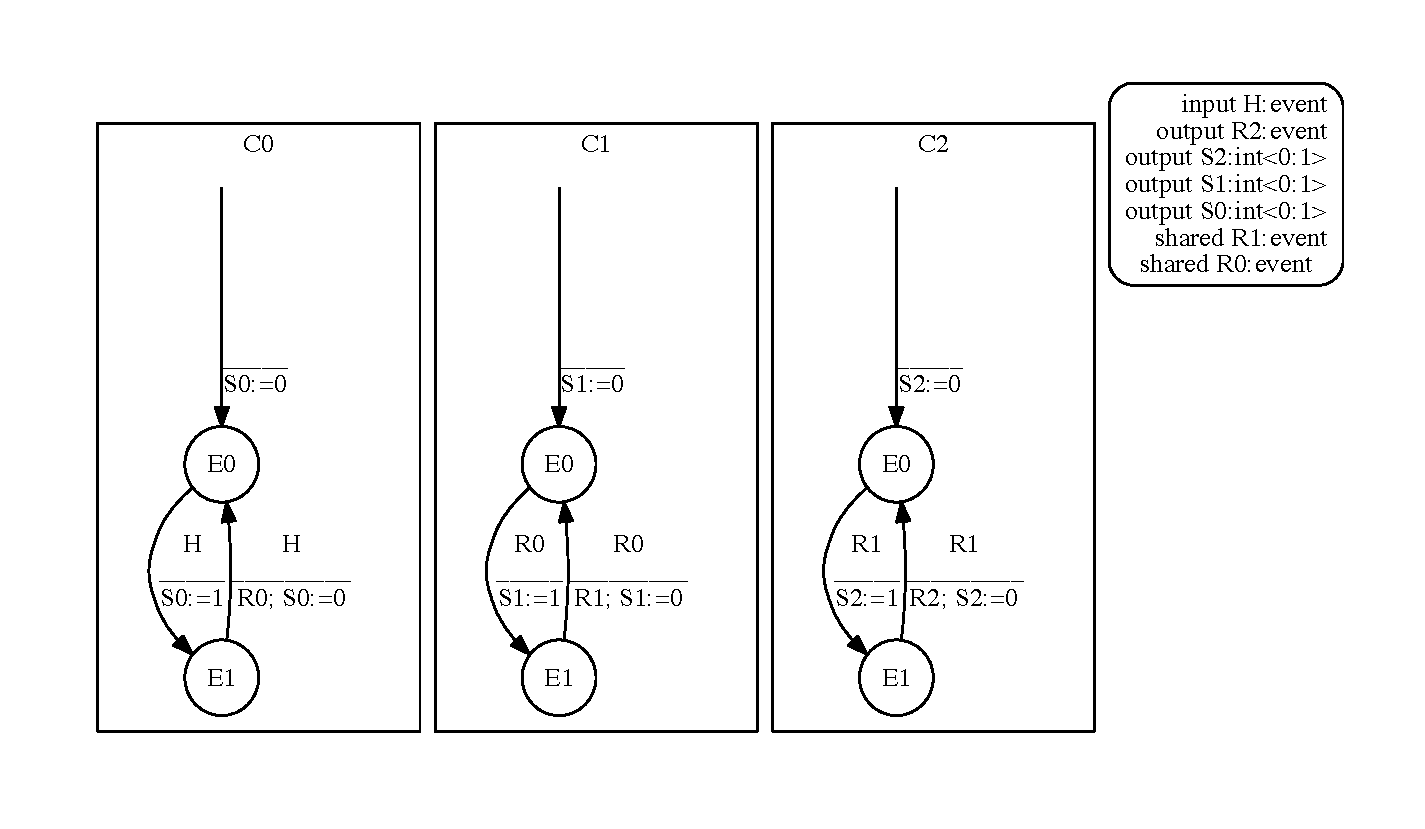
\includegraphics[height=9cm]{figs/ctrmod8-top}
   \centering
  \caption{A graphical representation of program described in Listing~\ref{lst:rfsm-cntmod8}}
  \label{fig:rfsm-cntmod8-top}
\end{figure}

\clearpage
\begin{figure}[!h]
   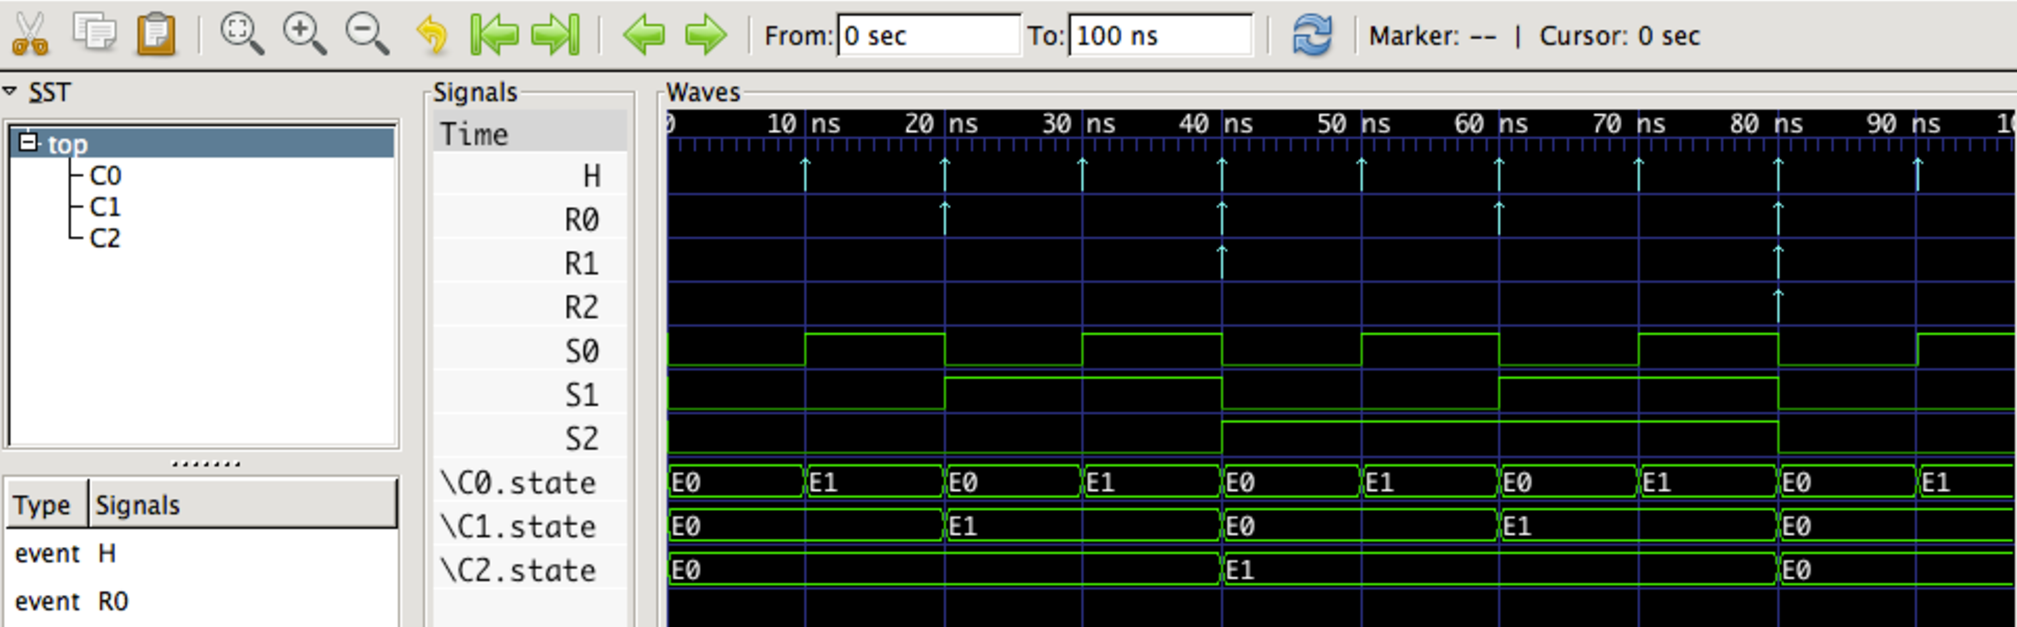
\includegraphics[width=\textwidth]{figs/ctrmod8-chrono}
   \centering
  \caption{Simulation results for the program in Listing~\ref{lst:rfsm-cntmod8}}
  \label{fig:rfsm-cntmod8-vcd}
\end{figure}

\subsection{Functions}
\label{sec:functions}

Conditions and actions associated to FSM transitions can use globally defined functions. An example
is given in listing~\ref{lst:rfsm-heron}\footnote{This example can be found in directory
  \texttt{examples/heron/v2} in the distribution.}. The FSM described here computes an approximation
of its input \verb|u| using Heron's classical algorithm. Successive approximations are computed in
state \verb|Iter| and the end of computation is detected when the square of the current
approximation \verb|x| differs from the argument (\verb|a|) from less than a given threshold
\verb|eps|. For this, the model uses the global function \verb|f_abs| defined at the beginning of
the program. This function computes the absolute value of its argument and is used twice in the
definition of the FSM model \verb|heron|, for defining the condition associated to the two
transitions going out of state \verb|Iter|.

\begin{lstlisting}[language=Rfsm,frame=single,numbers=left,caption=An RFSM program using a global
  function definition,label={lst:rfsm-heron},float]
function f_abs(x: float) : float { return x < 0.0 ? -.x : x }

fsm model Heron<eps: float>(
  in h: event,
  in start: bool,
  in u: float,
  out rdy: bool,
  out niter: int,
  out r: float)
{
  states: Idle, Iter;
  vars: a: float, x: float, n: int;
  trans:
  | Idle -> Iter on h when start=1 with a:=u, x:=u, rdy:=0, n:=0
  | Iter -> Iter on h when f_abs(x*.x-.a)>=eps with x:=(x+.a/.x)/.2.,
                                                    n:=n+1
  | Iter -> Idle on h when f_abs(x*.x-.a)<eps with r:=x, niter:=n, rdy:=1;
  itrans:
  | -> Idle with rdy:=1;
}

input H : event = periodic (10,10,200)
input U : float = value_changes (5:2.0)
input Start : bool = value_changes (0:0, 25:1, 35:0)
output Rdy : bool
output R : float
output niter : int

fsm heron = Heron<0.00000001> (H,Start,U,Rdy,niter,R)
\end{lstlisting}

\medskip
\step The general form for a function definition is 

\begin{center}
\framebox{\lstinline[language=Rfsm]| function name (<arg\_1>:<type\_1>, ..., <arg\_n>:<type\_n>)\ :\ <type\_r> \{ return <expr> \}|}
\end{center}

\noindent
where
\begin{itemize}
\item \lstinline[language=Rfsm]|<arg_i>| (resp. \lstinline[language=Rfsm]|<type_i>|) is the name
  (resp. type) of the i$^{th}$ argument,
\item \lstinline[language=Rfsm]|<type_r>| is the type of value returned by the function,
\item \lstinline[language=Rfsm]|<expr>| is the expression defining the function value.
\end{itemize}

\medskip
\step Functions can only return one result and cannot use local variables. There are therefore more
like so-called \emph{macros} in the C language than full-fledged functions and are typically used to
improve readability of the programs.

\clearpage
\subsection{Constants}
\label{sec:constants}

Global constants can be defined using the following syntax~:  

\begin{center}
\framebox{\lstinline[language=Rfsm]|constant name : <type> = <value>|}
\end{center}

\noindent
where
\begin{itemize}
\item \lstinline[language=Rfsm]|<type>| is the type of the defined constant (currently limited to
  \verb|int|, \verb|float| and arrays of \verb|int|s or \verb|float|s,
\item \lstinline[language=Rfsm]|<value>| is the value of the constant (which must be an \verb|int|
  or \verb|float| literal or an array of such literals).
\end{itemize}

Global constants, just like global functions, have a global scope and hence can be used in any FSM
model or instance.

\subsection{Semantic issues}
\label{sec:semantic-issues}

This presentation of the language has deliberately focused on syntax. Formalizing the semantics of programs made of
reactive finite state machines -- and in particular when several of these machines are interacting
-- is actually far from trivial and will not be carried out here. 

Instead, this section will describe some ``practical'' problems that may arise when simulating such
systems and how the language currently addresses them, without delving too much into the underlying
semantics issues\footnote{This is not that these issues do not deserve a formal treatment. Of
  course, they do ! But we think we this document is not the right place to do it.}.

\subsubsection{Priorities}
\label{sec:priorities}

The FSM models involved in programs should normally be \emph{deterministic}. In other words, a
situation where several transitions are enabled at the same instant should normally never arise. But
this condition may actually be difficult to enforce, especially for models reacting to several input
events. Consider for example, the model described in Listing~\ref{lst:rfsm-prio-pb}. This model
describes a (simplified) stopwatch. It starts counting seconds (materialized by event \verb|sec|)
as soon as event \verb|startstop| occurs and stops as soon as it occurs again.

\begin{lstlisting}[language=Rfsm,frame=single,numbers=left,caption=A program showing a potentially non-deterministic
  model,label={lst:rfsm-prio-pb},float]
fsm model chrono (
     in sec: event,
     in startstop: event,
    out aff: int)
  {
  states: Stopped, Running;
  vars: ctr: int;
  trans:
  | Stopped -> Running on startstop with ctr:=0; aff:=0
  | Running -> Running on sec with ctr:=ctr+1; aff:=ctr
  | Running -> Stopped on startstop;
  itrans:
  |-> Stopped;
  }

input StartStop: event = sporadic(25,70)
input H:event = periodic(10,10,110)
output Aff: int

fsm c = chrono(H,StartStop,Aff)
\end{lstlisting}

The problem is that if both events occur simultaneously  then
both the transitions at line 10 and 11 are enabled. In fact, here's the error message produced by
the compiler when trying to simulate the above program :

\small
\begin{verbatim}
Error when simulating FSM c: non deterministic transitions found at t=70:
	- Running--h|ctr:=ctr+1; aff:=ctr->Running[0]
	- Running--startstop->Stopped[0]
\end{verbatim}
\normalsize

Of course, this could be avoided by modifying the stimuli attached to input \verb|StartStop| so that the
corresponding events are never emitted at time $t=n\times 10$. But this is, in a sence, cheating,
since this event is supposed to modelize user interaction which occur, by essence, at impredictible
dates. 

The above problem can be solved by assigning a \emph{priority} to transitions. In the current
implementation, this is achieved by tagging some transitions as ``high priority''
transitions\footnote{Future versions may evolve towards a more sophisticated mechanism allowing
  numeric priorities.}.  When several transitions are enabled, if one is tagged as ``high priority''
than it is automatically selected\footnote{If none (resp. several) is (resp. are) tagged, the
  conflict remains, of course.}. 

Syntaxically, tagging a transition is simply achieved by replacing the leading ``\verb+|+'' by a
``\verb|!|''.  In the
case of the example above, the modified program is given in
Listing~\ref{lst:rfsm-prio-solved}. Tagging the last transition is here equivalent to give to the
\verb|startstop| precedence against the \verb|h| event when the model is in state
\verb|Running|.

\begin{lstlisting}[language=Rfsm,frame=single,numbers=left,caption=A rewriting of the model defined
  in Listing~\ref{lst:rfsm-prio-pb}, label={lst:rfsm-prio-solved},float]
fsm model chrono (...)
  {
  ...
  trans:
    ...
    | Running -> Running on sec with ctr:=ctr+1; aff:=ctr
    ! Running -> Stopped on startstop
  itrans: -> Stopped;
  }
...
\end{lstlisting}

\subsubsection{Sequential vs. synchronous actions}
\label{sec:sequ-vs.-synchr}

An important question is whether, when a transition specifying \emph{several actions} to be
performed is taken, the corresponding actions are performed sequentially or not. 

Consider for example, the following transition, in which \verb|x| and \verb|y| are internal
variables of the enclosing FSM :

\begin{center}
\example{\lstinline[language=Rfsm]'S0 -> S1 on H with x:=x+1, y:=x*2'}
\end{center}

Suppose that the value of variable \verb|x| is 1 just before event \verb|H| occurs. What will the value of
variables \verb|x| and \verb|y| after this transition ?

\step With a \textbf{sequential interpretation}, actions are performed sequentially, one after the
other, in the order they are specified. With this interpretation, order of execution matters. In the example above, it will
assign the value 2 to \verb|x| and 4 to \verb|y|.

\step With a \textbf{synchronous interpretation}, actions are performed in parallel, the value of each variable
occuring in right-hand-side expressions being the one \emph{before} the transition. With this
interpretation, order of executions does \emph{not} matter. In the example above, it will
assign the value 2 to \verb|x| and 2 to \verb|y|.

\medskip
A sequential interpretation naturally fits a software execution model, in which FSM variables are
implemented as program variables and actions as immediate modifications of these variables, whereas
a synchronous interpretation reflects hardware execution models, in which FSM variables are
typically implemented as registers which are updated in parallel at each clock cycle.

\medskip
By default, the \verb|rfsmc| compiler relies on a sequential interpretation, both for simulation and
code production\footnote{For the C and SystemC backends, this means that FSM variables are
  implemented as local variables of the function implementing the FSM model. For the VHDL backend,
  these variables are implemented as \texttt{variable}s withing the process implementing the
  FSM.}. But, in certain cases, and in particular when specifying models to be synthetized on
hardware, a synchronous interpretation is more natural and/or can lead to more efficient
implementations. Switching to a synchronous interpretation is possible by invoking the \verb|rfsmc|
compiler with the \verb|-synchronous_actions| option\footnote{For the VHDL backend, in particular, the
  \texttt{-synchronous\_actions} option forces the FSM variables to be implemented as
  \texttt{signal}s.}.  

% \medskip
% \textbf{Note}. As a syntactic reminder, list of actions are printed in diagrams using ``\verb|;|'' as a separator when using
% a sequential interpretation and using ``\verb|,|'' when using a synchronous interpretation.

%%% Local Variables: 
%%% mode: latex
%%% TeX-master: "rfsm"
%%% End: 
